\documentclass[11pt]{article}

\usepackage[margin=1in]{geometry}
\usepackage{graphicx}
\usepackage[colorlinks=true,allcolors=blue]{hyperref}
\usepackage{authblk}
\usepackage[style=numeric, sorting=none, backend=biber]{biblatex}
\addbibresource{references.bib}



% determines the spacing and general formatting of each section in the document
\makeatletter
\renewcommand{\@maketitle}{%
    \newpage
    \null
    \vskip 2em%
    \let\footnote\thanks
    \begin{center}%
        {\LARGE \@title \par}%
    \end{center}%
        \vskip 1em%
        {\large \noindent\begin{minipage}{\textwidth}\raggedright \@author\end{minipage}\par}%
        \vskip 1em%
    \begin{center}%
        {\@date}%
    \end{center}%
    \par
    \vskip 1.5em%
}

% Compact bibliography format: [N] Author et al., Year, ShortJournal.
\DeclareNameFormat{familyonly}{%
  \ifnumequal{\value{listcount}}{1}{%
    \namepartfamily%
    \ifnumgreater{\value{listtotal}}{1}{ et al.}{}%
  }{}%
}
\DeclareBibliographyDriver{article}{%
  \printnames[familyonly]{author}%
  , \printfield{year}%
  , \printfield{shortjournal}%
  }
\DeclareBibliographyDriver{inproceedings}{%
  \printnames[familyonly]{author}%
  , \printfield{year}%
  , \printfield{shortjournal}%
}
\AtBeginBibliography{\setlength{\parskip}{0pt}}
\setlength{\bibitemsep}{0pt}
\setlength{\bibparsep}{0pt}

\makeatother

\title{Leveraging Eutectic Interfaces in Geodynamic models of Europa’s Ice shell to constrain Physical Parameters}
\renewcommand\Authands{, }
\author[1,2]{William Byrne}
\author[1]{Ana-Catalina Plesa}
\author[1]{Hauke Hussmann}
\author[3]{Dustin Schroeder}
\author[4]{Gregor Steinbr\"ugge}
\author[5]{Natalie Wolfenbarger}

\affil[1]{Institute of Space Research, German Aerospace Center (DLR), Berlin, Germany\\
\href{mailto:William.Byrne@dlr.de}{William.Byrne@dlr.de}; \href{mailto:Ana.Plesa@dlr.de}{Ana.Plesa@dlr.de}; \href{mailto:Hauke.Hussmann@dlr.de}{Hauke.Hussmann@dlr.de};}
\affil[2]{Freie Universit\"at Berlin, Berlin, Germany\\
\href{mailto:byrnew02@zedat.fu-berlin.de}{byrnew02@zedat.fu-berlin.de};}
\affil[3]{Department of Geophysics, Stanford University, Stanford, CA, USA\\
\href{mailto:Dustin.M.Schroeder@stanford.edu}{Dustin.M.Schroeder@stanford.edu}}
\affil[4]{Jet Propulsion Laboratory, California Institute of Technology, Pasadena, CA, USA\\
\href{mailto:gregor.b.steinbruegge@nasa.jpl.gov}{gregor.b.steinbruegge@nasa.jpl.gov}}
\affil[5]{Los Alamos National Laboratory, Los Alamos, NM, USA\\
\href{mailto:wolfenbarger@lanl.gov}{wolfenbarger@lanl.gov}}
\date{21.01.2026:\href{https://meetingorganizer.copernicus.org/EPSC-DPS2025/EPSC-DPS2025-1952.html}{View abstract on the EPSC2025 website}}


\begin{document}

\maketitle

\raggedright
\setlength{\parindent}{0pt}
\setlength{\parskip}{\baselineskip}

\section*{Abstract}

Jupiter’s moon Europa is one of the prime targets for planetary exploration due to its high astrobiological potential. Slightly smaller than Earth’s moon, Europa harbors a liquid water ocean beneath an ice shell. The thickness of Europa’s ice shell is poorly constrained and values of less than 1 km  to up to 90 km have been suggested in previous studies that investigated shell thickness via a combination of thermal, impact, and mechanical models \parencite{billingsGreatThicknessDebate2005,vilellaTidallyHeatedConvection2020}. Low thickness values were derived from mechanical models, which can generally only estimate the thickness of the brittle layer. Thermal and impact models can consider the entire ice shell and estimates using such models suggest the higher thickness end-member values.

Ice-penetrating radars on NASA’s Europa-CLIPPER (REASON, \parencite{blankenshipRadarEuropaAssessment2024}) and ESA’s JUICE (RIME, \parencite{bruzzoneRIMERadarIcy2013a}) missions aim to determine the thickness of Europa's ice shell. Recent studies have suggested that constraints on the thickness of Europa’s ice shell can be obtained through the detection of eutectic interfaces, defined as the depth where brine becomes thermodynamically stable in the ice shell \parencite{schroederConstrainingThicknessConductive2024}.  In fact, previous studies have shown that the detection of eutectic horizons within an ice shell is likely easier than detecting the ice-ocean interface, given their shallower depths and therefore lower total signal attenuation \parencite{kalousovaRadarAttenuationEuropas2017,soucekRadarAttenuationEnceladus2023,byrneRadarAttenuationSubsurface2024}. The depth of the eutectic interfaces depends on the thermal state of the ice shell, which is closely linked to the ice shell viscosity and large-scale dynamics \parencite{kalousovaRadarAttenuationEuropas2017}. As suggested by previous authors \parencite{schroederConstrainingThicknessConductive2024,kalousovaRadarAttenuationEuropas2017}, detection of eutectic interfaces therefore represents a promising strategy to constrain the thermophysical properties of the ice shell through characterization of its convective pattern.

In this study we use the geodynamic code GAIA-v2 \parencite{huttigImprovedFormulationIncompressible2013} to investigate the ice shell dynamics on Europa. GAIA-v2 is a finite volume fluid flow solver. It numerically solves the conservation equations of mass, linear momentum, and thermal energy in order to determine the thermal state and fluid flow within the interior or planetary bodies. The code was originally developed to model solid-state convection in the interior of rocky bodies \parencite{laneuville13, tosi13b, plesaLargeScaleNumerical2016}, but was recently adapted to treat large-scale dynamics in the ice shell of moons in the outer solar system \parencite{ruckriemen2023move, Plesa20233}.

We vary the ice shell thickness and ice shell viscosity that largely affect the convection pattern and in particular the number of hot upwellings and cold downwellings that can develop. In our models, we use a 2D cylindrical geometry. While free-slip is implemented as a condition on all boundaries, the top layer naturally arrives at a no-slip boundary condition due to the strong temperature-dependent viscosity (which follows an Arrhenius law). We choose a reference value for the viscosity at the ice-ocean interface and vary this over several orders of magnitude between the different models. We set the surface temperature to the temperature at the equator of Europa (110 K), and the temperature at the base of our model to the melting temperature of water-ice at the respective pressure. In our simulations, we only include diffusion creep as a deformation mechanism and vary the reference viscosity over several orders of magnitude.

\begin{figure}[htbp]
\noindent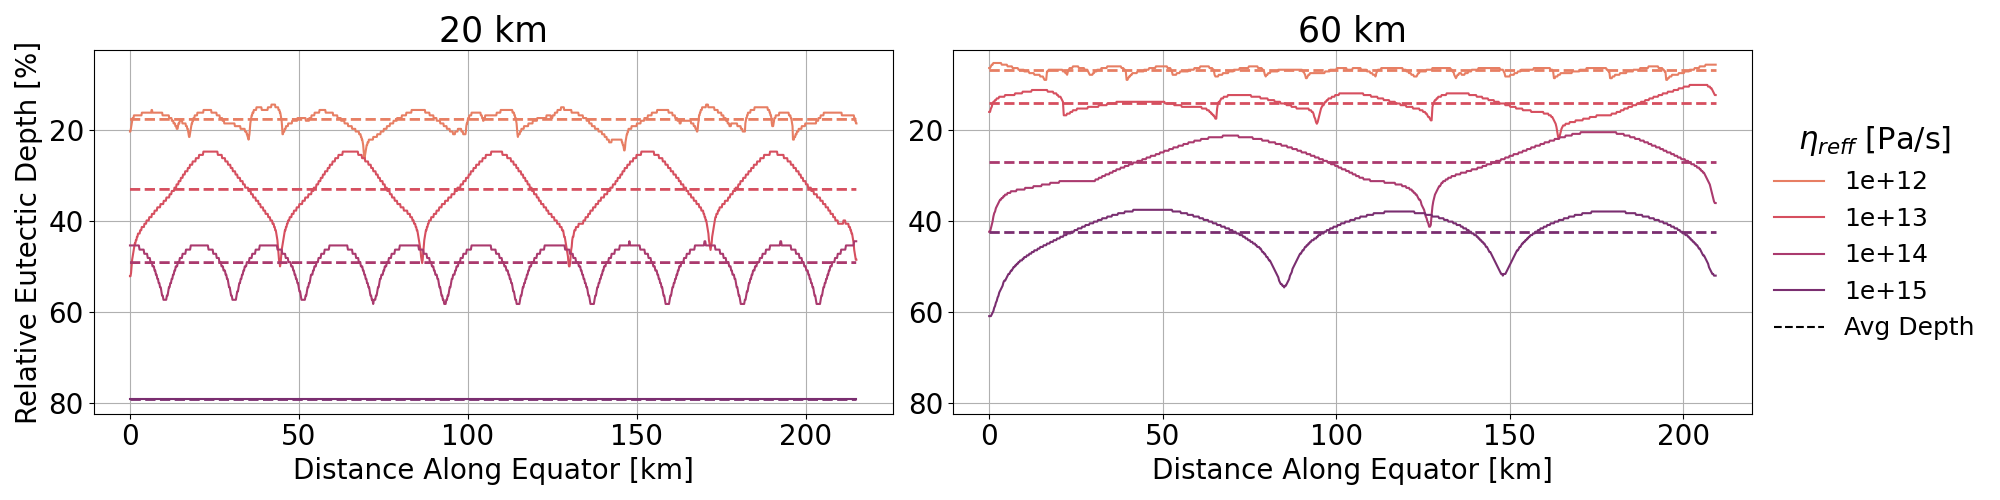
\includegraphics[width=\textwidth]{abstract_figures/epsc2025_fig1.png}
\caption{End-member Zoltov and Shock eutectic interfaces (237 K) for simulations with 20 km ice shell (left) and 60 km (right), varying reference viscosity by color. The dashed line represents the average eutectic depth (km) for the given eutectic interface.}
\label{fig1}
\end{figure}

Once a simulation has reached a statistical (quasi-)steady state, we determine the eutectic pattern by identifying the depths of the eutectic temperature. We treat this sequence of eutectic depths as a signal (Figure 1) and identify key characteristics of the interface like the number and location of upwellings and downwellings (peaks and troughs), average eutectic depth, and dominant signal frequency. The number of local maxima and minima are used in conjunction with the dominant frequency to estimate the global number of convective cells in the ice shell. Once these key characteristics are determined, we use them to develop scaling laws to key geodynamic parameters.

\begin{figure}[htbp]
\noindent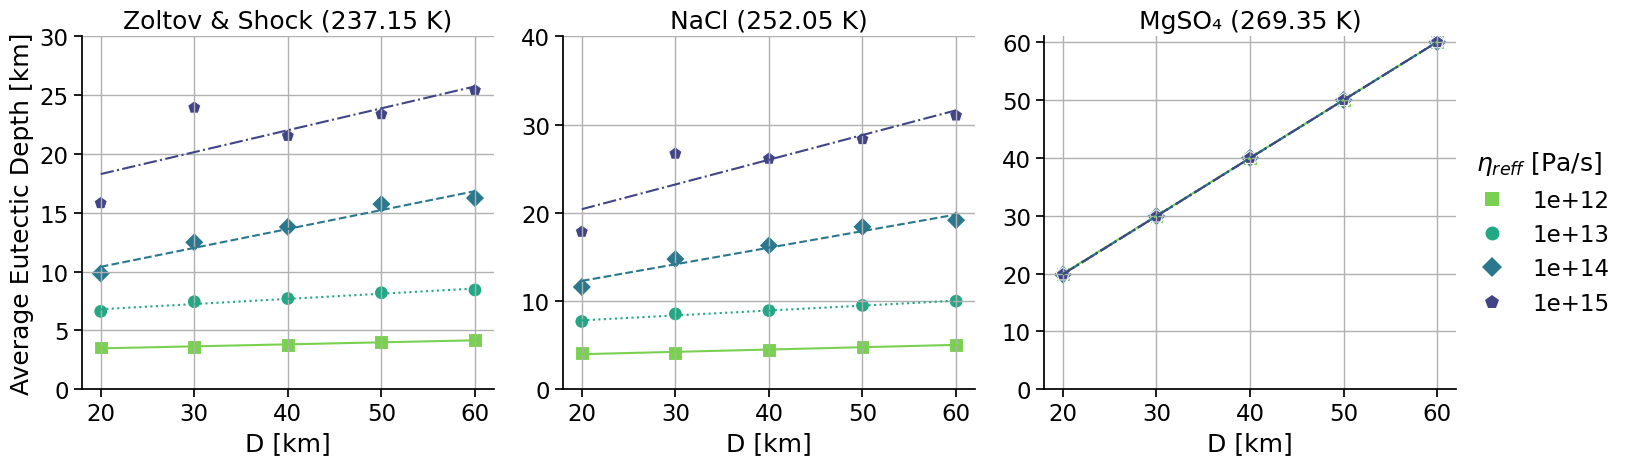
\includegraphics[width=\textwidth]{abstract_figures/epsc2025_fig2.png}
\caption{Ice shell thickness (D, km) plotted against average eutectic depth (km) for each simulation, for each eutectic temperature. A consistent positive relationship holds between Ice shell thickness and average eutectic depth for all simulations and the two colder eutectic temperatures. The eutectic temperature for MgSO4 is so close to the pressure-dependent solidus of water ice (ice-ocean interface temperature) that the average eutectic temperature will consistently be equivalent to ice shell depth.}
\label{fig2}
\end{figure}


While our preliminary results have struggled to demonstrate consistent relationships between global convective cell count and viscosity, they do show a close relation between the average eutectic depth and the total ice shell depth (Figure 2). By increasing the number and complexity of our simulations, we aim to fully develop these initial scaling laws which relate the convection structure with the viscosity and thickness of Europa’s ice shell. This will provide a framework that will help to interpret the detection of eutectic interfaces in future radar measurements in the context of large-scale dynamics of the deep ice shell. In future work, we will evaluate the ability to reconstructure patterns of the ice shell by using sparse radar echoes by analyzing cases of melt detection on terrestrial glaciers, and create a more realistic signal resolution based on terrestrial and non-terrestrial sounding studies.

\printbibliography[title={References}]

\end{document}
